\chapter{Definición de la Arquitectura Tecnológica}
\section{Identificación de las Necesidades de Infraesturctura Tecnológica}
Para llevar a cabo el desarrollo de la aplicación de turismo en Asturias, es fundamental identificar las necesidades de infraestructura tecnológica. Dado que la empresa no cuenta con ningún sistema en la actualidad, se hace necesario mencionar algunas de las necesidades básicas para llevar a cabo este proyecto.\\[1ex]Primero de todo se ha de escoger el modelo arquitectónico. En este caso se ha optado por un modelo cliente-servidor.\\[1ex]
\begin{figure}[H]
	\centering
	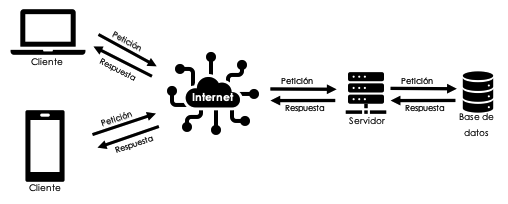
\includegraphics[width=13cm]{2-DefinicionDeLaArquitecturaTecnologica/arquitectura.png}
	\caption{Modelo cliente-servidor}
\end{figure}
Este modelo es el más básico y consiste en un cliente que se comunica con un servidor para acceder a los datos. En este caso, el cliente sería la aplicación, y el servidor sería el encargado de manejar la base de datos y la lógica de negocio.
Para implementarlo, es necesario realizar un análisis exhaustivo de las diferentes opciones tecnológicas disponibles para el desarrollo de la aplicación y para el servidor
\subsection{Aplicación web y móvil}
Para el desarrollo de esta aplicación hay varias alternativas. Entre ellas podemos destacar la realización de aplicaciones nativas, web apps o aplicaciones híbridas~\cite{nativas_vs_web_vs_hibridas}~\cite{web_vs_nativas_vs_hibridas}.
\subsubsection{Aplicaciones Nativas}
Las aplicaciones nativas se desarrollan específicamente para un sistema operativo concreto, utilizando su SDK correspondiente. Esto les permite acceder de manera óptima a las funcionalidades del dispositivo y ofrecen un alto rendimiento y una mejor experiencia de usuario. Por ejemplo, para iOS se utiliza Swift y para Android, Kotlin o Java son las opciones más comunes. La desventaja es que requieren un desarrollo separado para cada plataforma, lo que puede aumentar los costes y tiempos de desarrollo.
\subsubsection{Web Apps}
Las aplicaciones web se ejecutan en un navegador y están desarrolladas principalmente en HTML5, CSS y JavaScript. No necesitan ser instaladas en el dispositivo y son accesibles desde cualquier plataforma con acceso a internet. Son más económicas y rápidas de desarrollar en comparación con las aplicaciones nativas y funcionan en casi todos los dispositivos. Sin embargo, suelen depender de una buena conexión a internet y pueden no ofrecer la misma fluidez y acceso a funciones del dispositivo que una aplicación nativa.
\subsubsection{Aplicaciones Híbridas}
Las aplicaciones híbridas combinan elementos de las aplicaciones nativas y web. Se desarrollan utilizando tecnologías web pero se empaquetan dentro de un contenedor nativo, permitiéndoles acceder a las funcionalidades del dispositivo. Esto significa que se puede escribir el código una sola vez y adaptarlo a múltiples plataformas. Ejemplos notables de aplicaciones híbridas incluyen Instagram y Airbnb ~\cite{airbnb}. Sin embargo, su rendimiento es menor en comparación con las nativas y se pueden encontrar posibles complejidades cuando se requiere acceso a funcionalidades específicas del dispositivo.\\[1ex]
Sin embargo, es importante tener en cuenta que, a pesar de las ventajas en términos de desarrollo multiplataforma, el rendimiento de las aplicaciones híbridas puede ser menor en comparación con las puramente nativas y pueden surgir complejidades cuando se requiere acceso a funcionalidades específicas del dispositivo.\\[1ex]
Para facilitar el desarrollo de aplicaciones híbridas, existen varios frameworks que ofrecen un conjunto de herramientas y componentes reutilizables. Estos frameworks permiten a los desarrolladores centrarse en la lógica y funcionalidad de la aplicación, reduciendo el tiempo y esfuerzo necesario para desarrollar aplicaciones que funcionen en múltiples plataformas. A continuación, revisamos algunos de los frameworks más populares ~\cite{ionic_vs_native_vs_fluter}:
\begin{itemize}
	\item \textbf{Ionic:} Utiliza tecnologías web como HTML, CSS y JavaScript para construir aplicaciones móviles. Esto significa que puedes aprovechar tus habilidades web existentes y reutilizar código en diferentes plataformas. Ionic también cuenta con una robusta biblioteca de componentes de UI, gestos y herramientas para construir una aplicación con apariencia nativa.
	\item \textbf{React Native:} Utiliza tecnologías web pero compila el código a componentes nativos, por lo que el rendimiento y la experiencia son muy cercanos a los de una aplicación nativa. Tiene una gran colección de bibliotecas de terceros e integraciones. Sin embargo, puede ser más difícil de aprender en comparación con Ionic y Flutter. React Native también cuenta con el respaldo de Facebook, por lo que tiene una comunidad y un ecosistema fuertes.
	\item \textbf{Flutter:} Flutter utiliza el lenguaje de programación Dart de Google y widgets propietarios, y renderiza todo usando Skia, un motor de renderizado 2D. Esto permite que las aplicaciones de Flutter logren una apariencia y sensación nativas con alto rendimiento. Flutter es un framework relativamente nuevo, pero está creciendo rápidamente con una comunidad fuerte y muchas bibliotecas y plugins disponibles. Sin embargo, Dart puede tener una curva de aprendizaje más pronunciada para aquellos que vienen de los lenguajes web.
\end{itemize}
\subsection{Servidor}
En el desarrollo del backend, se dispone de una amplia gama de tecnologías que nos permiten construir y gestionar la lógica y los datos de nuestra aplicación.
\subsubsection{Framework y Entorno}
\begin{itemize}
	\item \textbf{Spring Boot:} Framework de Java muy valorado por su capacidad de simplificar el desarrollo de aplicaciones empresariales y microservicios. Ofrece autoconfiguración, una vasta colección de módulos y herramientas que permiten el desarrollo eficiente, y es compatible con diversas tecnologías de bases de datos tanto SQL como NoSQL. Su arquitectura basada en microservicios favorece la escalabilidad y flexibilidad, y su robusta documentación apoya a los desarrolladores a lo largo del proceso de desarrollo. Además, gracias a su naturaleza políglota y al soporte de la JVM, Spring Boot se integra bien con otros lenguajes de programación, ofreciendo una gran versatilidad para proyectos diversos~\cite{spring_boot_framework}.
	\item \textbf{NodeJS:} Entorno de ejecución que utiliza JavaScript para el desarrollo del backend. Es adecuado para un amplio rango de aplicaciones, desde aplicaciones en tiempo real, Internet de las Cosas (IoT) y aplicaciones basadas en REST API. NodeJS es reconocido por su eficiencia en el manejo de múltiples conexiones simultáneas, su capacidad para escalar aplicaciones, y por ser parte de un ecosistema rico en módulos y bibliotecas disponibles a través de NPM. Esto lo hace ideal para aplicaciones que requieren actualizaciones en tiempo real y para el desarrollo ágil y eficiente, manteniendo las operaciones no bloqueantes y basadas en eventos. Además, su comunidad de desarrollo activa y creciente ofrece un gran soporte y continua innovación~\cite{node_js}.
\end{itemize}
\subsubsection{Base de datos}
Tras elegir el framework y entorno adecuados para nuestro backend, es crucial seleccionar una base de datos que no solo se alinee con la naturaleza de nuestra aplicación, sino que también ofrezca el rendimiento, escalabilidad y fiabilidad necesarios. Las bases de datos son el pilar sobre el cual se estructuran, almacenan y acceden los datos esenciales para la funcionalidad de la aplicación.
\begin{itemize}
	\item \textbf{Relacional:} Es un tipo de base de datos que almacena y proporciona acceso a puntos de datos relacionados entre sí. Se basan en el modelo relacional, una forma intuitiva y directa de representar datos en tablas. Además, soportan transacciones ACID (Atomicidad, Consistencia, Aislamiento, Durabilidad), lo que garantiza que las operaciones de la base de datos se realicen de manera confiable y segura.\\
	      Sin embargo, las bases de datos relacionales pueden ser menos flexibles en términos de datos no estructurados o variables y es necesario añadir más potencia a un único servidor en caso de que aumente la demanda~\cite{sql}.
	\item \textbf{No relacional:} Es un tipo de base de datos que se caracteriza por su capacidad para almacenar y manejar grandes volúmenes de datos distribuidos, su esquema flexible y su escalabilidad horizontal. Hay muchos tipos de bases de datos, pero la que más se enfoca a este proyecto es la de documentos. En ella se asocia cada clave con una estructura de datos compleja llamada 'documento'. Estas bases de datos son idóneas para manejar datos semiestructurados y no estructurados ya que permiten una gran flexibilidad en la estructura de los datos almacenado. Algunos ejemplos de bases de datos de documentos son MongoDB~\cite{mongodb} y Couchbase~\cite{couchbase}.
	      Sin embargo, es importante considerar que las bases de datos NoSQL, a pesar de su escalabilidad y flexibilidad, pueden presentar desafíos en términos de consistencia de datos y complejidad de las consultas~\cite{nosql}.
\end{itemize}
\section{Selección de la arquitectura tecnológica}
Tras una exhaustiva evaluación de las distintas arquitecturas de aplicaciones móviles, se ha optado por el desarrollo de aplicaciones híbridas como la estrategia principal para este proyecto. Las aplicaciones híbridas, que integran las ventajas de las aplicaciones web y nativas, nos permiten escribir un único código base que es adaptable a múltiples plataformas, reduciendo significativamente el tiempo y los costos asociados con el desarrollo y mantenimiento en iOS y Android.\\[1ex]Hemos optado por la combinación de React e Ionic frente a otras alternativas como React Native y Flutter, basándonos en consideraciones estratégicas y en la experiencia previa del equipo. Si bien React Native es una poderosa solución para el desarrollo de aplicaciones móviles con capacidades para la web, su enfoque principal se centra en el desarrollo móvil. Sin embargo, la sinergia de React con Ionic se orienta específicamente hacia el desarrollo de aplicaciones híbridas desde su concepción, facilitando una experiencia de desarrollo unificada tanto para plataformas móviles como web. \\[1ex]La decisión de no elegir Flutter se basó principalmente en la curva de aprendizaje asociada con el dominio de Dart, el lenguaje de programación utilizado por Flutter, lo cual representa un desafío adicional para el equipo.\\[1ex]Para complementar nuestra elección de tecnologías frontend, hemos decidido adoptar un stack MERN~\cite{mern}. La integración de Node.js con Express.js para el desarrollo de nuestra API REST, junto con una base de datos NoSQL de documentos, ofrece una solución cohesiva y eficiente. Esta combinación no solo aprovecha la experiencia del equipo en tecnologías web, sino que también asegura una arquitectura escalable y flexible.